\documentclass[a4paper,14pt]{article}

%%% Работа с русским языком
\usepackage[english,russian]{babel}   %% загружает пакет многоязыковой вёрстки
\usepackage{fontspec}      %% подготавливает загрузку шрифтов Open Type, True Type и др.
\defaultfontfeatures{Ligatures={TeX},Renderer=Basic}  %% свойства шрифтов по умолчанию
\setmainfont[Ligatures={TeX,Historic}]{Times New Roman} %% задаёт основной шрифт документа
\setsansfont{Arial}                    %% задаёт шрифт без засечек
\setmonofont{Courier New}
\usepackage{indentfirst}
\frenchspacing

%%% Дополнительная работа с математикой
\usepackage{amsmath,amsfonts,amssymb,amsthm,mathtools} % AMS
\usepackage{icomma} % "Умная" запятая: $0,2$ --- число, $0, 2$ --- перечисление

\renewcommand{\epsilon}{\ensuremath{\varepsilon}}
\renewcommand{\phi}{\ensuremath{\varphi}}
\renewcommand{\kappa}{\ensuremath{\varkappa}}
\renewcommand{\le}{\ensuremath{\leqslant}}
\renewcommand{\leq}{\ensuremath{\leqslant}}
\renewcommand{\ge}{\ensuremath{\geqslant}}
\renewcommand{\geq}{\ensuremath{\geqslant}}
\renewcommand{\emptyset}{\varnothing}

%%% Работа с картинками
\usepackage{graphicx}  % Для вставки рисунков
\graphicspath{%
	{images/equally-spaced-arrays},
	{images/array-distributions-theory},
	{images/array-distributions-modeling},
	{images/interpolation},
	{images/iterative},
	{images/mimo},
}  % папки с картинками
%\usepackage{subfig}
\setlength\fboxsep{3pt} % Отступ рамки \fbox{} от рисунка
\setlength\fboxrule{1pt} % Толщина линий рамки \fbox{}
\usepackage{wrapfig} % Обтекание рисунков текстом
\usepackage[lflt]{floatflt}
\usepackage{subcaption}
\usepackage[labelfont=bf]{caption}
\captionsetup{justification=centering,singlelinecheck=false}
\renewcommand\thesubfigure{\asbuk{subfigure}}
\counterwithin{figure}{section}
\usepackage{float}

% Работа с графиками
\usepackage{tikz}
\usepackage{pgfplots}
\usepackage{pgfplotstable}

%%% Работа с таблицами
\usepackage{array,tabularx,tabulary,booktabs} % Дополнительная работа с таблицами
\counterwithin{table}{section}
%%%%%%%%%%%%%%%%%%%%%%%%%%%%%%%%%%%%%%%%%%%%%%%%%%%%%%%%%%%%%%%%%%%%%%%%
\usepackage{tabularray}
\DefTblrTemplate{caption-tag}{default}{\textbf{\tablename\hspace{0.25em}\thetable}}
\DefTblrTemplate{caption-sep}{default}{\enskip}
\DefTblrTemplate{caption-text}{default}{\InsertTblrText{caption}}

\DefTblrTemplate{caption}{default}{
	\raggedleft
	\UseTblrTemplate{caption-tag}{default}
	\UseTblrTemplate{caption-sep}{default}
	\UseTblrTemplate{caption-text}{default}

}

\DefTblrTemplate{contfoot-text}{default}{Продолжение на следующей странице}
\SetTblrTemplate{contfoot-text}{default}

\DefTblrTemplate{conthead-text}{default}{(Продолжение)}

\DefTblrTemplate{conthead}{default}{
	\UseTblrTemplate{conthead-text}{default}
}

\DefTblrTemplate{capcont}{default}{
	\hfill
	\UseTblrTemplate{caption-tag}{default}
	\UseTblrTemplate{caption-sep}{default}
	\UseTblrTemplate{caption-text}{default}
	\UseTblrTemplate{conthead-text}{default}
}
%%%%%%%%%%%%%%%%%%%%%%%%%%%%%%%%%%%%%%%%%%%%%%%%%%%%%%%
\usepackage{multirow} % Слияние строк в таблице
\usepackage{array}

%%% Программирование
\usepackage{tcolorbox}
\usepackage{etoolbox} % логические операторы

%%% Страница
\usepackage{extsizes} % Возможность сделать 14-й шрифт
\usepackage{geometry}
\geometry{top=20mm}
\geometry{bottom=20mm}
\geometry{left=30mm}
\geometry{right=15mm}
%%%
\righthyphenmin=2

%%% Настройка отображения содержания
\usepackage{tocloft}
\renewcommand{\cftpartleader}{\cftdotfill{\cftdotsep}} % for parts
\renewcommand{\cftsecleader}{\cftdotfill{\cftdotsep}} % for sections
%%% Заголовки
\usepackage{titlesec}
\titleformat{\section}{\Large\normalfont\bfseries\raggedright}{\arabic{section}.}{0.5ex}{}
\titleformat{\subsection}{\large\normalfont\bfseries\raggedright}{\arabic{section}.\arabic{subsection}.}{0.5ex}{}
\titleformat{\subsubsection}{\normalfont\bfseries\raggedright}{\arabic{section}.\arabic{subsection}.\arabic{subsubsection}.}{0.5ex}{}
\titlespacing*{\section}{0pt}{\baselineskip}{\baselineskip}

\providecommand\phantomsection{}
%\newcommand\schap[1]{\chapter*{#1} \addcontentsline{toc}{chapter}{#1} \phantomsection}
\newcommand\ssect[1]{\section*{#1} \phantomsection \addcontentsline{toc}{section}{#1} \markboth{#1}{#1}}
\newcommand{\rwn}{\the\numexpr\value{rownum}-1\relax}
%%% Custom appendix naming
\usepackage[toc,page]{appendix}
\renewcommand\appendixname{Приложение}
\renewcommand\appendixpagename{Приложения}
\renewcommand\appendixtocname{Приложения}



%%% Ссылки
%\usepackage[superscript]{cite} % Ссылки в верхних индексах
%\usepackage[nocompress]{cite} % 
\usepackage{csquotes} % Еще инструменты для ссылок
%\renewcommand{\refname}{Список источников}
%\addto\captionsrussian{\def\refname{Список источников}}

\usepackage[%
	backend=biber,% движок
	bibencoding=utf8,% кодировка bib файла
	sorting=none,% настройка сортировки списка литературы
	style=gost-numeric,% стиль цитирования и библиографии (по ГОСТ)
	language=autobib,% получение языка из babel/polyglossia, default: autobib % если ставить autocite или auto, то цитаты в тексте с указанием страницы, получат указание страницы на языке оригинала
	autolang=other,% многоязычная библиография
	clearlang=true,% внутренний сброс поля language, если он совпадает с языком из babel/polyglossia
	defernumbers=true,% нумерация проставляется после двух компиляций, зато позволяет выцеплять библиографию по ключевым словам и нумеровать не из большего списка
	sortcites=true,% сортировать номера затекстовых ссылок при цитировании (если в квадратных скобках несколько ссылок, то отображаться будут отсортированно, а не абы как)
	doi=false,% Показывать или нет ссылки на DOI
	isbn=false,% Показывать или нет ISBN, ISSN, ISRN
	mincitenames=3,
	maxcitenames=3,
	maxbibnames=3,
]{biblatex}

\addbibresource{include/references.bib}

\DefineBibliographyStrings{russian}{%
	bibliography = {Список источников},
}

%\renewcommand{\baselinestretch}{1.15}
%\usepackage{setspace} % Интерлиньяж
%\spacing{1.15}
%\onehalfspacing % Интерлиньяж 1.5
%\doublespacing % Интерлиньяж 2
%\singlespacing % Интерлиньяж 1

\usepackage{lastpage} % Узнать, сколько всего страниц в документе.


\usepackage{soul} % Модификаторы начертания
\usepackage{hyperref}
\hypersetup{%
	colorlinks=true,
	linkcolor=blue,
	filecolor=magenta,
	urlcolor=cyan,
	pdfauthor={Лазба Филипп},
	pdftitle={Магистерская диссертация на тему «исследование методов оптимизации современных антенных решеток»},
	pdfsubject={Исследование методов оптимизации современных антенных решеток},
	pdfkeywords={АФАР; ЦАР; AESA; DAA; антенные решётки},
	bookmarks=true,
	pdfpagemode=UseThumbs,
}


%\renewcommand{\familydefault}{\sfdefault} % Начертание шрифта

\usepackage{multicol} % Несколько колонок




\renewcommand{\epsilon}{\ensuremath{\varepsilon}}
\renewcommand{\phi}{\ensuremath{\varphi}}
\renewcommand{\kappa}{\ensuremath{\varkappa}}
\renewcommand{\le}{\ensuremath{\leqslant}}
\renewcommand{\leq}{\ensuremath{\leqslant}}
\renewcommand{\ge}{\ensuremath{\geqslant}}
\renewcommand{\geq}{\ensuremath{\geqslant}}
\renewcommand{\emptyset}{\varnothing}

\newcommand{\bhline}[1]{\noalign{\hrule height #1pt}}



\renewcommand{\theenumii}{\arabic{enumi}.}
\renewcommand{\theenumii}{\arabic{enumi}.\arabic{enumii}}
\renewcommand{\theenumiii}{\arabic{enumi}.\arabic{enumii}.\arabic{enumiii}}

% \usepackage{xassoccnt}
% \NewTotalDocumentCounter{totalfigures}
% \NewTotalDocumentCounter{totaltables}
% \DeclareAssociatedCounters{figure}{totalfigures}
% \DeclareAssociatedCounters{table}{totaltables}

% \usepackage{listings}
% \usepackage{matlab-prettifier}

\usepackage{minted}
\usemintedstyle{friendly_grayscale}
\renewcommand\theFancyVerbLine{\normalsize\arabic{FancyVerbLine}}

%%%%%%%%%%%%%%%%%%%%%%%%%%%%%%%%%%%%%%%%%%%%%%%%%%%%%%%%%%%%%%%

\newcommand*{\figoneendian}{\totalfigures~рисунок}
\newcommand*{\figfourendian}{\totalfigures~рисунка}
\newcommand*{\figfiveendian}{\totalfigures~рисунков}

% Расчёт значений для общего числа рисунков
\newcommand*{\printtotfig}[1][,]{%
	\newbool{less11Q}%
	\newbool{greater19Q}%
	\boolfalse{less11Q}%
	\boolfalse{greater19Q}%
	\newcounter{Ptempnumexpr}%
	\newcounter{Pwordindex}%
	\setcounter{Ptempnumexpr}{0}%
	\addtocounter{Ptempnumexpr}{\numexpr\totalfigures-100*(\totalfigures/100)}%
	\ifnumequal{\totalfigures}{-1}%
	{??#1}%
	{\ifnumequal{\totalfigures}{0}{}%
		{\ifnumless{\value{Ptempnumexpr}}{11}{\booltrue{less11Q}}{}%
			\ifnumgreater{\value{Ptempnumexpr}}{19}{\booltrue{greater19Q}}{}%
			\ifboolexpr{bool {less11Q} or bool {greater19Q}}%
			{\setcounter{Pwordindex}{0}%
				\addtocounter{Pwordindex}{\numexpr\value{Ptempnumexpr}-10*(\value{Ptempnumexpr}/10)}%
				\ifnumequal{\value{Pwordindex}}{1}% Окончание для 1
				{\figoneendian}%
				{\ifnumequal{\value{Pwordindex}}{2}% Окончание для 4
					{\figfourendian}%
					{\ifnumequal{\value{Pwordindex}}{3}%
						{\figfourendian#1}%
						{\ifnumequal{\value{Pwordindex}}{4}%
							{\figfourendian}%
							{\figfiveendian}% Окончание для 5
						}%
					}%
				}%
			}%
			{\figfiveendian}% Окончане для 5
		}%
	}%
}

\usepackage[figure,table]{totalcount}

\author{Лазба Филипп}
\title{}
\date{\today}

\renewcommand{\baselinestretch}{1.15} % put the factor in the second argument 
\usepackage{ragged2e}
\justifying{}

\begin{document}
	\thispagestyle{empty}
\setcounter{page}{1}

\begin{center}
    МИНОБРНАУКИ РОССИИ

    \vspace{1ex}

    Федеральное государственное автономное образовательное учреждение 
    
    высшего образования

    \textbf{НАЦИОНАЛЬНЫЙ ИССЛЕДОВАТЕЛЬСКИЙ УНИВЕРСИТЕТ <<МОСКОВСКИЙ ИНСТИТУТ ЭЛЕКТРОННОЙ ТЕХНИКИ>>}

    \vspace{1ex}

    Институт микроприборов и систем управления
\end{center}

\vspace{17ex}

\begin{center}
    Лазба Филипп Борисович 
    
    \vspace{1ex}
    \textbf{Магистреская диссертация}

    по направлению
    \textbf{\textit{11.04.01 <<Радиотехника>>}}
    
    \vspace{1ex}
    \textit{Исследование методов оптимизации современных антенных решеток}

\end{center}

\vspace{25ex}

% \begin{longtblr}[
% 	caption = {Основные параметры SPF5043Z},
% 	label = {table:LNA-parameters}
% 	]{
% 		colspec={Q[1,l,m]Q[1,l,m]},width=\textwidth,
% 		vlines,hlines,
% 		vspan=even,
% 		rowhead=1,
% 		row{1}={font=\bfseries}
% 	}
% 	%%%%%%%%%%%%%%%%%%%%%%%%%%%%%%%%%%%%%%%%%%%%%%%
% 	Параметр & Значение \\
% 	%%%%%%%%%%%%%%%%%%%%%%%%%%%%%%%%%%%%%%%%%%%%%%%%
% 	Усиление & 18,2 дБ \\
% 	Коэффициент шума & 0,7 дБ \\
% 	Точка однодецибельной компрессии & 22,6 дБмВт \\
% 	Размеры ШхДхВ & 2х2х1 мм \\
% \end{longtblr}

\SetTblrTemplate{caption}{empty}

\begin{longtblr}[
  ]{
    colspec = {Q[l] Q[c] Q[r]},
    row{odd} = {m},
    row{even} = {m}
  }
  Студент   & \SetCell[r=1]{c}\underline{\hspace{5cm}} & Лазба Ф.Б. \\
  Руководитель   & & \\
  к.т.н., доцент & \SetCell[r=1]{c}\underline{\hspace{5cm}} & Орешкин В.И. \\
            & & \\
\end{longtblr}

\SetTblrTemplate{caption}{default}

\vfill

\begin{center}
    Москва, Зеленоград

    2024
\end{center}

\newpage
	
	{\Large\normalfont\bfseries \hfil Аннотация}
\vspace{1em}
\thispagestyle{empty}

Магистерская диссертация на тему «исследование методов оптимизации современных антенных решеток».

Работа состоит из введения, 5 глав, заключения, списка источников и приложений.

В работе рассмотрены существующие подходы к решению задач оптимизации антенных решёток и 
особенности их реализации; проведено моделирование, на основе которого были сделаны выводы.

В заключении приведены выводы и итог проведённого исследования.

Работа содержит~\pageref*{LastPage} страниц, 2~таблицы, \printtotfig.
Для написания данной работы было использовано 33 источника. 

\ 

{\Large\normalfont\bfseries \hfil Annotation}
\vspace{1em}
\thispagestyle{empty}

Master's thesis on the topic "research of optimization methods for modern antenna arrays".

The work consists of an introduction, 5 chapters, a conclusion, a list of sources and appendices.

The paper considers existing approaches to solving antenna array optimization problems and the features of
their implementation; modeling is carried out, on the basis of which conclusions were drawn.

In conclusion, results of the study are presented.

The work contains~\pageref*{LastPage} pages, 2~tables, \totalfigures~figures. 
A total of 33 sources were used to write this work.

	\tableofcontents{}
	\ssect{Список терминов и сокращений}

{
\noindent \textbf{АР} --- антенная решётка

\noindent \textbf{ФАР} --- фазированная антенная решётка

\noindent \textbf{АФАР} --- активная фазированная антенная решётка

\noindent \textbf{РНС} --- радионавигационная система

\noindent \textbf{ЦАР} --- цифровая антенная решётка

\noindent \textbf{ДН} --- диаграмма направленности

\noindent \textbf{ДНА} --- диаграмма направленности антенны

\noindent \textbf{УБЛ} --- уровень боковых лепестков

\noindent \textbf{УДЛ} --- уровень дифракционных лепестков

\noindent \textbf{ШГЛ} --- ширина главного лепестка
}
	\ssect{Введение}\label{chap:introduction}

Антенные решётки играют важную роль во многих сферах современной жизни. Их применение можно увидеть, например, в следующих областях:

\begin{itemize}
      \item Системы радиосвязи
            \begin{itemize}
                  \item В базовых станциях мобильной связи для создания узких областей покрытия, что помогает
                        обеспечивать связь в труднодоступных зонах и осуществлять пространственное
                        разделение в густонаселенных районах, что позволяет увеличить пропускную способность
                  \item В системах спутниковой связи для осуществления покрытия сигналом больших областей
                        и улучшения качества связи за счёт создания узких, но быстро перестраиваемых диаграмм направленности.
            \end{itemize}
      \item Радиолокационные системы
            \begin{itemize}
                  \item Применение антенных решёток в военных, авиационных и автомобильных радарах позволяет быстро сканировать пространство
                        и эффективно обнаруживать объекты и вычислять их параметры (местоположение, скорость и направление движения);
                        осуществлять слежение за быстро передвигающимися целями и принимать решения на основе полученных данных.
            \end{itemize}
      \item Радиоастрономия
            \begin{itemize}
                  \item В радиотелескопах, таких как Very Large Array (VLA), для изучения космических
                        радиоволн, исходящих от различных астрономических объектов.
            \end{itemize}
\end{itemize}

Несмотря на свои многочисленные достоинства, активные фазированные антенные решётки обладают такими недостатками
как сложность разработки, возможные большие размеры и высокая стоимость. В зависимости от области применения инженерам
приходится находить оптимальные соотношения между сложностью, стоимостью, скоростью сканирования, размерами, ремонтопригодностью
и многими другими параметрами антенных решёток, которые противоречат друг другу. Ввиду большого количества учитываемых параметров,
многокритериальная оптимизация требует комплексного подхода и глубокого понимания взаимодействия между ними.


Цель данной магистерской работы заключается в проведении обзора существующих методов оптимизации антенных решёток с последующим анализом и сравнением их эффективности.

Задачами данной работы являются:

\begin{itemize}
      \item Исследовать различные геометрические и амплитудно-фазовые распределения
      \item Исследовать метод итеративной обработки данных
      \item Исследовать возможности применения интерполяции в антенных решётках
      \item Исследовать применения технологии MIMO в радиолокаторах
\end{itemize}

Работа направлена на исследование того, как различные методы оптимизации могут влиять на важные параметры системы - такие как сложность, стоимость,
размер и скорость сканирования. На основе проведённого анализа будет сформулирован ряд рекомендаций по выбору и
применению методов в зависимости от специфики задачи и условий эксплуатации.
	\section{Антенные решётки с равномерным распределением амплитуд и межэлементных расстояний}\label{chap:equally-spaced-arrays}

Основополагающие принципы фазированных антенных решёток были заложены ещё в 1905 году Карлом Фердинандом Брауном,
который получил Нобелевскую премию по физике за разработку методов управления направленностью антенн
с помощью фазового сдвига. Однако широкое применение и разработка таких антенн начались только в середине 20-го века.
Технология начала активно развиваться в 1950-1960х годах в рамках военных и космических программ.
Первые практические применения антенных решёток были связаны с радиолокационными системами для отслеживания
воздушных и космических объектов. 

Классические ФАР представляют собой массив антенных элементов с одинаковыми характеристиками и синфазной запиткой,
расположенными равномерно в линии или на плоскости. Принцип работы ФАР заключается в управлении фазами волн
в антенных элементах таким образом, чтобы через синфазное сложение этих волн с/в определённом направлении достигалось
усиление сигнала, тогда как в других -- ослабление.

На Рисунке~\ref{fig:equally-spaced-distribution} 
показано расположение элементов линейной антенной решётке
и полученные диаграммы направленности в нескольких направлениях

\begin{figure}[!ht]
	\centering
	\begin{subfigure}[b]{0.8\textwidth}
		\centering
		
\includegraphics[width=\textwidth]{equally-spaced-distribution.png}
		\caption{}%
		\label{fig:equally-spaced-distribution-pos}
	\end{subfigure}
	\begin{subfigure}[b]{0.55\textwidth}
		\centering
		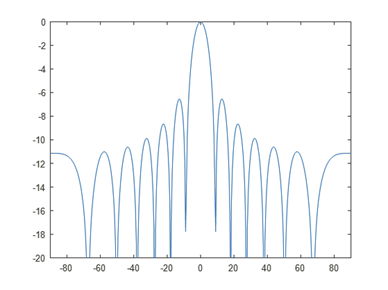
\includegraphics[width=\textwidth]{equally-spaced-distribution-beam-pattern0.png}
		\caption{}%
		\label{fig:equally-spaced-distribution-beam-pattern0}
	\end{subfigure}
	\hfill
	\begin{subfigure}[b]{0.49\textwidth}
		\centering
		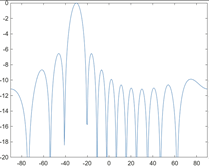
\includegraphics[width=\textwidth]{equally-spaced-distribution-beam-pattern-30.png}
		\caption{}%
		\label{fig:equally-spaced-distribution-beam-pattern-30}
	\end{subfigure}
	\begin{subfigure}[b]{0.49\textwidth}
		\centering
		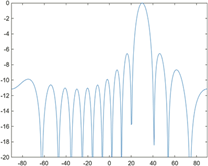
\includegraphics[width=\textwidth]{equally-spaced-distribution-beam-pattern30.png}
		\caption{}%
		\label{fig:equally-spaced-distribution-beam-pattern30}
	\end{subfigure}
	\caption{%
	(а) Расположение элементов 
	ДН при направленности на 
	(б) 0 
	(в) -30 и 
	(г) +30 градусов
	}%
	\label{fig:equally-spaced-distribution}
\end{figure}

Такие антенные решётки применяются и в современных приложениях ввиду простоты их разработки, однако имеют
несколько недостатков: высокий уровень боковых лепестков
(на Рисунке~\ref{fig:equally-spaced-distribution-beam-pattern0}
видно, что уровень второго лепестка составляет порядка -7 дб от основного), увеличение стоимости ввиду
большого количества  элементов, которое требуется для поддержания требуемой ширины основного лепестка при
расстоянии между элементами $d \leq \lambda/2$, либо появление 
дифракционных лепестков (ложных целей) при увеличении межэлементного расстояния,
которое можно увидеть на Рисунке~\ref{fig:equally-spaced-distribution-granting-lobes}

\begin{figure}[ht]
	\centering
	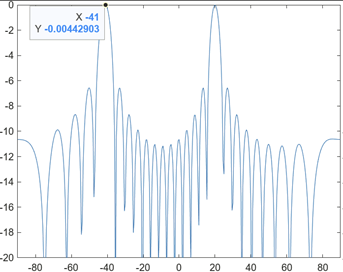
\includegraphics[width=0.8\textwidth,keepaspectratio]{equally-spaced-distribution-granting-lobes.png}
	\caption{ДН при межэлементном расстоянии $d > \lambda/2$, 
	направленность на~20~градусов,
	дифракционный лепесток~на~-41~градус}%
	\label{fig:equally-spaced-distribution-granting-lobes}
\end{figure}

Такие решетки могут применяться в системах, где отсутствие множественной направленности менее критично чем
больший размер/вес итогового устройства, например в системах межспутниковой связи. Кроме того важную роль
играет простота разработки и наладки таких ФАР. 

В системах же, где эти параметры являются критичными, а также в тех случаях когда есть возможность применять
более сложные структуры, применяются решётки, разработанные с помощью методов, которые описаны в следующих
главах.

	\nocite{*}
\printbibliography[title={Список использованных источников},heading=bibintoc]
\end{document}